% ------------------------------------------------
\StartChapter{Methodology: GemGNN Framework}{chapter:methodology}
% ------------------------------------------------

\section{Framework Overview}

The GemGNN (Generative Multi-view Interaction Graph Neural Networks) framework addresses the fundamental challenges of few-shot fake news detection through a novel heterogeneous graph-based approach that eliminates dependency on user propagation data while maintaining the benefits of social context modeling. Our architecture represents a systematic solution to three critical limitations in existing approaches: (1) the unavailability of real user interaction data due to privacy constraints, (2) the poor performance of existing methods in few-shot scenarios, and (3) the lack of rigorous evaluation protocols that prevent information leakage between training and test sets.

\begin{figure}[h]
    \centering
    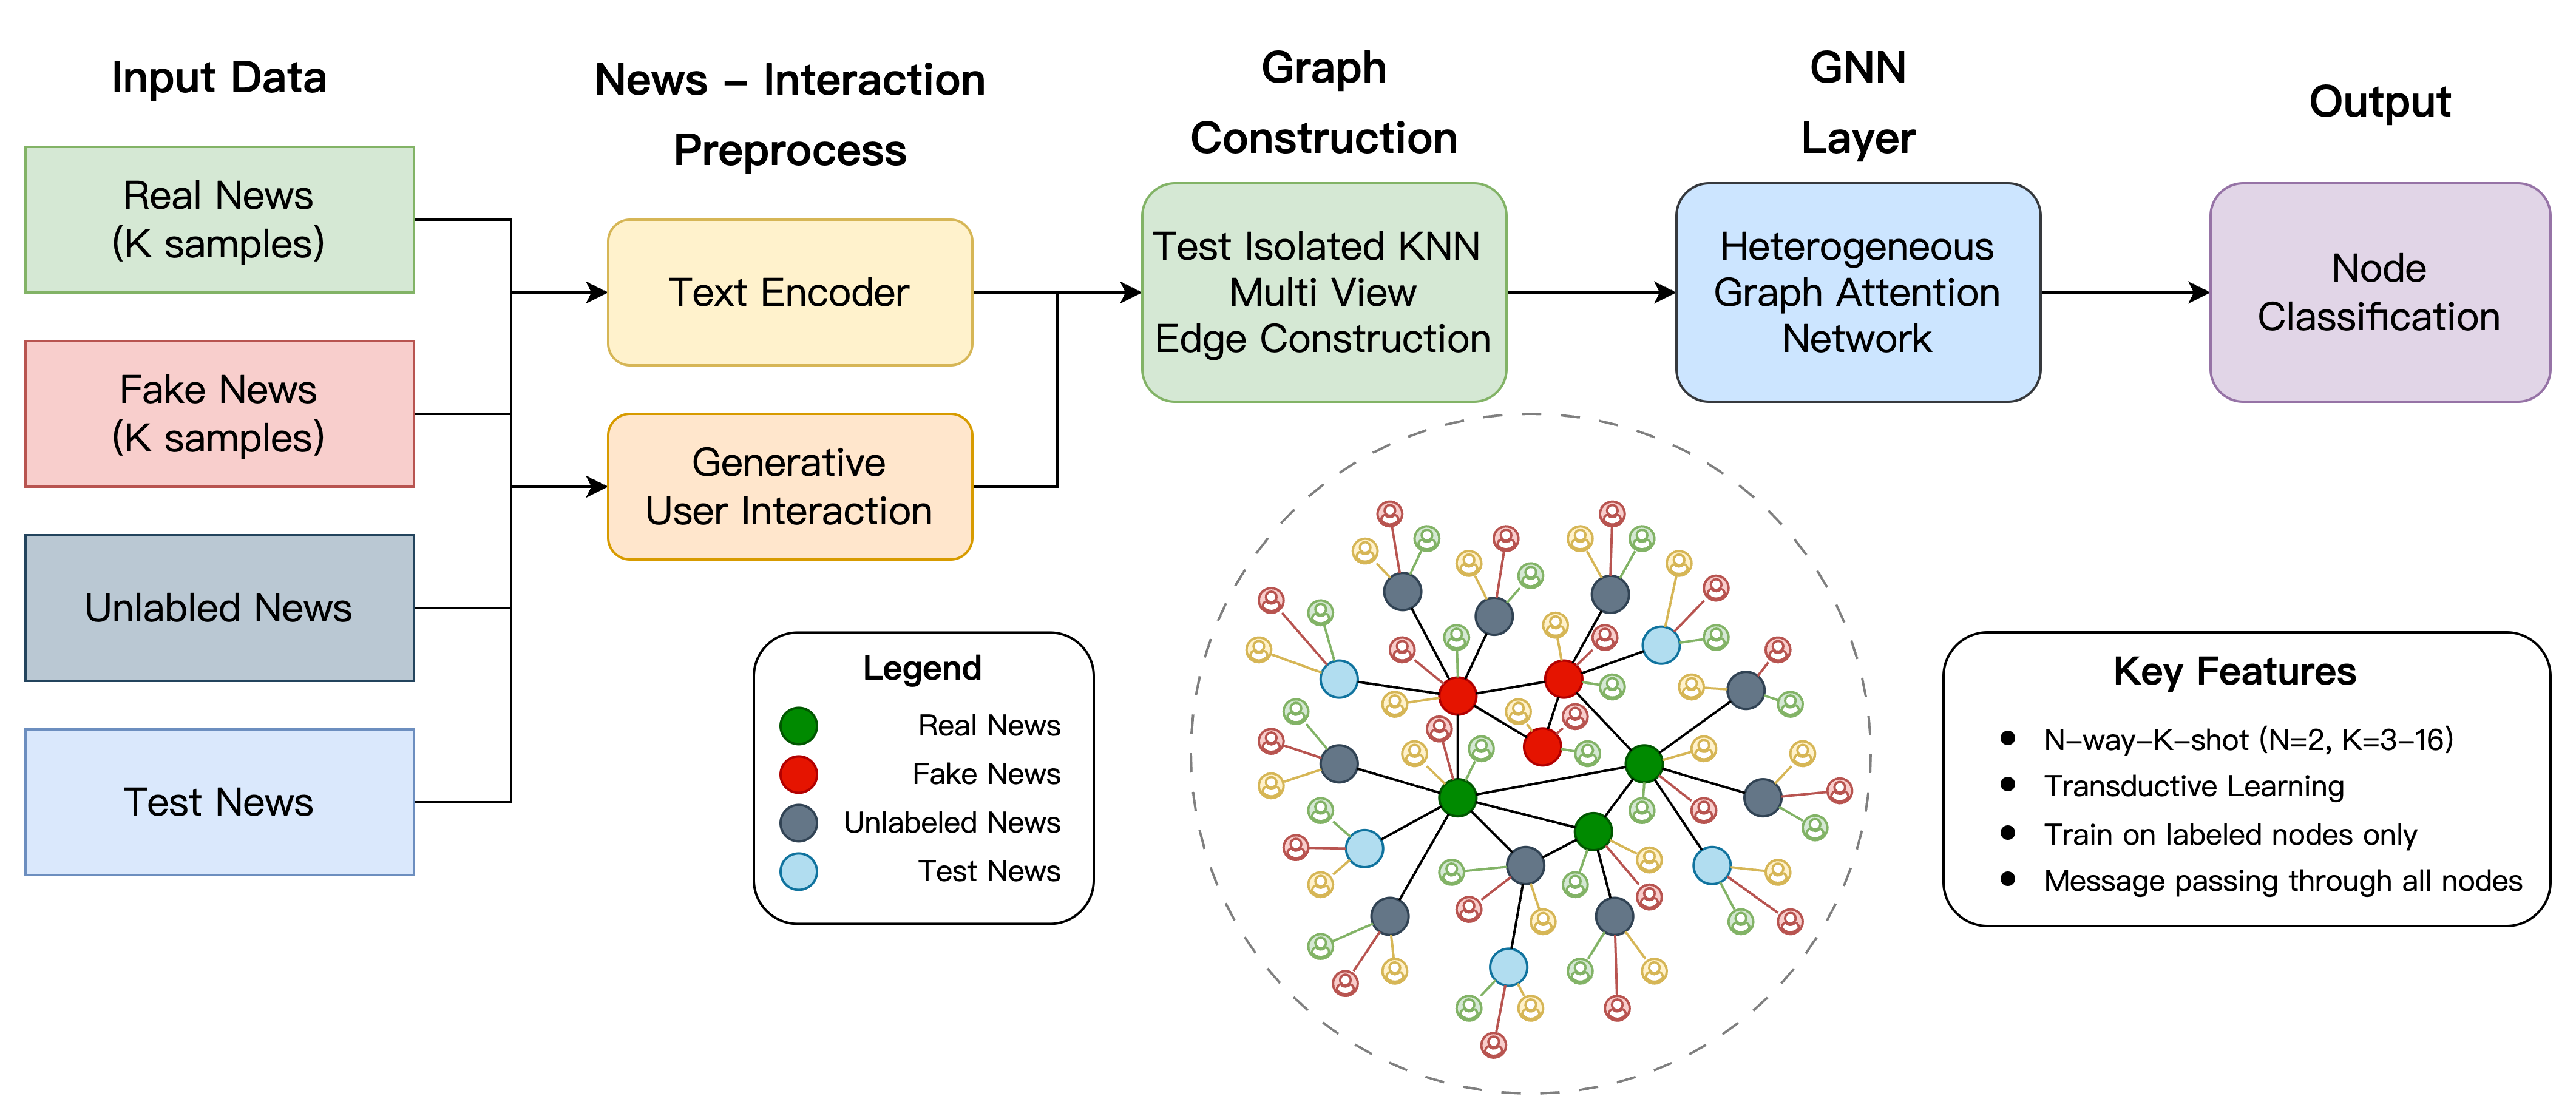
\includegraphics[width=0.8\textwidth]{context/methodology/fig/pipeline.png}
    \caption{Complete GemGNN pipeline showing data flow from news articles through heterogeneous graph construction to final classification}
    \label{fig:pipeline}
\end{figure}

The complete architecture consists of four interconnected components that work synergistically to achieve robust few-shot performance (see Figure~\ref{fig:pipeline}): (1) \emph{Generative User Interaction Simulation} using Google's Gemini LLM to create realistic social context without privacy concerns, (2) \emph{Adaptive Graph Construction} with configurable edge policies (traditional KNN vs test-isolated KNN) to balance performance optimization with evaluation realism, (3) \emph{Multi-View Graph Architecture} that leverages DeBERTa's disentangled attention structure to capture complementary semantic perspectives, and (4) \emph{Heterogeneous Graph Neural Network} with enhanced training strategies specifically designed for few-shot learning scenarios.

\textbf{Core Design Philosophy:} Our approach operates under a transductive learning paradigm where all nodes (labeled, unlabeled, and test) participate in heterogeneous message passing, but only labeled nodes contribute to loss computation. This design philosophy maximizes the utility of limited supervision by leveraging the heterogeneous graph structure to propagate information from labeled news nodes to unlabeled and test nodes through learned type-specific attention mechanisms. The framework maintains strict separation between training and test data when required, while allowing flexible adaptation to different deployment scenarios through configurable graph construction policies.

\textbf{Implementation Architecture:} The framework is implemented through two primary components that reflect our systematic approach to heterogeneous graph construction and training. The \texttt{HeteroGraphBuilder} class (implemented in \texttt{build\_hetero\_graph.py}) handles the complete pipeline from news article processing through heterogeneous graph construction, while the training pipeline (implemented in \texttt{train\_hetero\_graph.py}) provides specialized few-shot learning strategies including enhanced loss functions, early stopping criteria, and comprehensive evaluation protocols.

Our approach begins with pre-trained DeBERTa embeddings~\cite{he2021deberta} for news articles, which provide rich semantic representations (768-dimensional vectors) that capture contextual relationships and linguistic patterns indicative of misinformation. These embeddings serve as the foundation for both similarity-based graph construction and node feature initialization in our heterogeneous graph neural network, ensuring that the model can leverage state-of-the-art natural language understanding capabilities within the graph-based architecture.

\section{Dataset Sampling Strategy}

A critical aspect of our methodology is the systematic approach to sampling training data that ensures balanced and effective few-shot learning. Our sampling strategy is designed to maximize the utility of limited labeled data while providing sufficient unlabeled context for effective transductive learning. The implementation in \texttt{HeteroGraphBuilder} provides multiple sampling configurations to address different few-shot learning scenarios and deployment constraints.

\subsection{Labeled Node Sampling}

For k-shot learning scenarios, we sample exactly k labeled examples per class from the training set, following established few-shot learning protocols~\cite{wang2020fewshot, finn2017model}. The sampling process uses the \texttt{sample\_k\_shot} utility function to ensure balanced representation:
\begin{itemize}
    \item \textbf{k real news articles}: Selected randomly from authentic news samples using stratified sampling
    \item \textbf{k fake news articles}: Selected randomly from misinformation samples with matched sampling
\end{itemize}

This balanced sampling ensures that the model receives equal representation from both classes during training, which is crucial for effective few-shot learning where class imbalance can severely impact performance. Our implementation supports k-shot values ranging from 3 to 16, with 8-shot being the primary evaluation setting based on empirical validation.

\subsection{Unlabeled Node Sampling with Multiple Strategies}

To leverage the transductive learning paradigm effectively, we implement multiple strategies for sampling additional unlabeled training nodes that participate in message passing but do not contribute to loss computation. The \texttt{HeteroGraphBuilder} supports three distinct unlabeled sampling approaches:

\textbf{Standard Uniform Sampling:} The default approach samples unlabeled nodes uniformly from the remaining training set. The number of unlabeled nodes is determined by:
\begin{equation}
N_{unlabeled} = \text{num\_classes} \times k \times \text{sample\_unlabeled\_factor}
\end{equation}

Where \texttt{sample\_unlabeled\_factor} defaults to 5, creating substantial unlabeled context (e.g., 80 unlabeled nodes in an 8-shot scenario: $2 \times 8 \times 5 = 80$).

\textbf{Pseudo-Label-Aware Sampling:} When \texttt{pseudo\_label=True}, the system employs confidence-based sampling that leverages pre-computed pseudo-labels and confidence scores. This approach sorts unlabeled instances by prediction confidence within each pseudo-label group and samples the most confident examples. The pseudo-label cache system (\texttt{pseudo\_label\_cache\_path}) enables consistent sampling across multiple experimental runs.

\textbf{Partial Unlabeled Sampling:} The \texttt{partial\_unlabeled} flag enables selective unlabeled sampling that focuses on high-quality instances based on embedding similarity to labeled examples. This strategy improves graph connectivity quality by ensuring that unlabeled nodes provide meaningful structural information for message passing.

This comprehensive sampling strategy ensures that the model has access to substantial unlabeled context while maintaining computational efficiency. The unlabeled nodes provide crucial structural information for graph-based message passing and help the model learn better representations through the heterogeneous graph architecture.

\subsection{Test Set Inclusion}

All available test set instances are included in the graph construction process. This comprehensive inclusion ensures:
\begin{itemize}
    \item \textbf{Realistic evaluation}: Test nodes represent the complete range of evaluation scenarios
    \item \textbf{Structural completeness}: The graph captures relationships between all relevant nodes
    \item \textbf{Transductive learning}: Test nodes benefit from message passing without contributing to training loss
\end{itemize}

The test nodes are connected to training nodes through the chosen edge construction strategy (traditional KNN or test-isolated KNN) but remain isolated from loss computation during training, maintaining the integrity of the few-shot evaluation protocol.

\section{Generative User Interaction Simulation}

Traditional propagation-based fake news detection methods rely on real user interaction data, which is often unavailable due to privacy constraints or platform limitations. To address this fundamental limitation, we introduce a novel generative approach that synthesizes realistic user interactions using Google's Gemini LLM. This approach represents a paradigm shift from dependency on actual social media data to controlled synthesis of social context.

\subsection{Gemini-based Interaction Generation Pipeline}

We employ Google's Gemini LLM through a systematic prompt engineering strategy to generate diverse user interactions for each news article. This approach addresses the limitations of traditional propagation-based methods~\cite{ma2016detecting, shu2017fake} that require real user interaction data. The generation process is designed to simulate authentic user responses that would naturally occur in social media environments, capturing the diversity of user reactions without privacy or access constraints.

For each news article $n_i$, we generate a set of user interactions $I_i = \{i_1, i_2, \ldots, i_{20}\}$ where each interaction represents a potential user response to the news content. The choice of 20 interactions per article balances computational efficiency with sufficient diversity to capture varied user perspectives. This systematic approach ensures consistent social context generation across all news articles in our datasets.

The prompt engineering strategy (see Figure~\ref{fig:prompt}) ensures that generated interactions reflect realistic user behavior patterns observed in social media platforms. We incorporate the complete news content, including headlines and article body, to generate contextually appropriate responses that capture various user perspectives and emotional reactions. The prompts are specifically designed to instruct Gemini to produce responses that vary in tone, perspective, and engagement level, mimicking the natural diversity of social media interactions.

\begin{figure}[h]
    \centering
    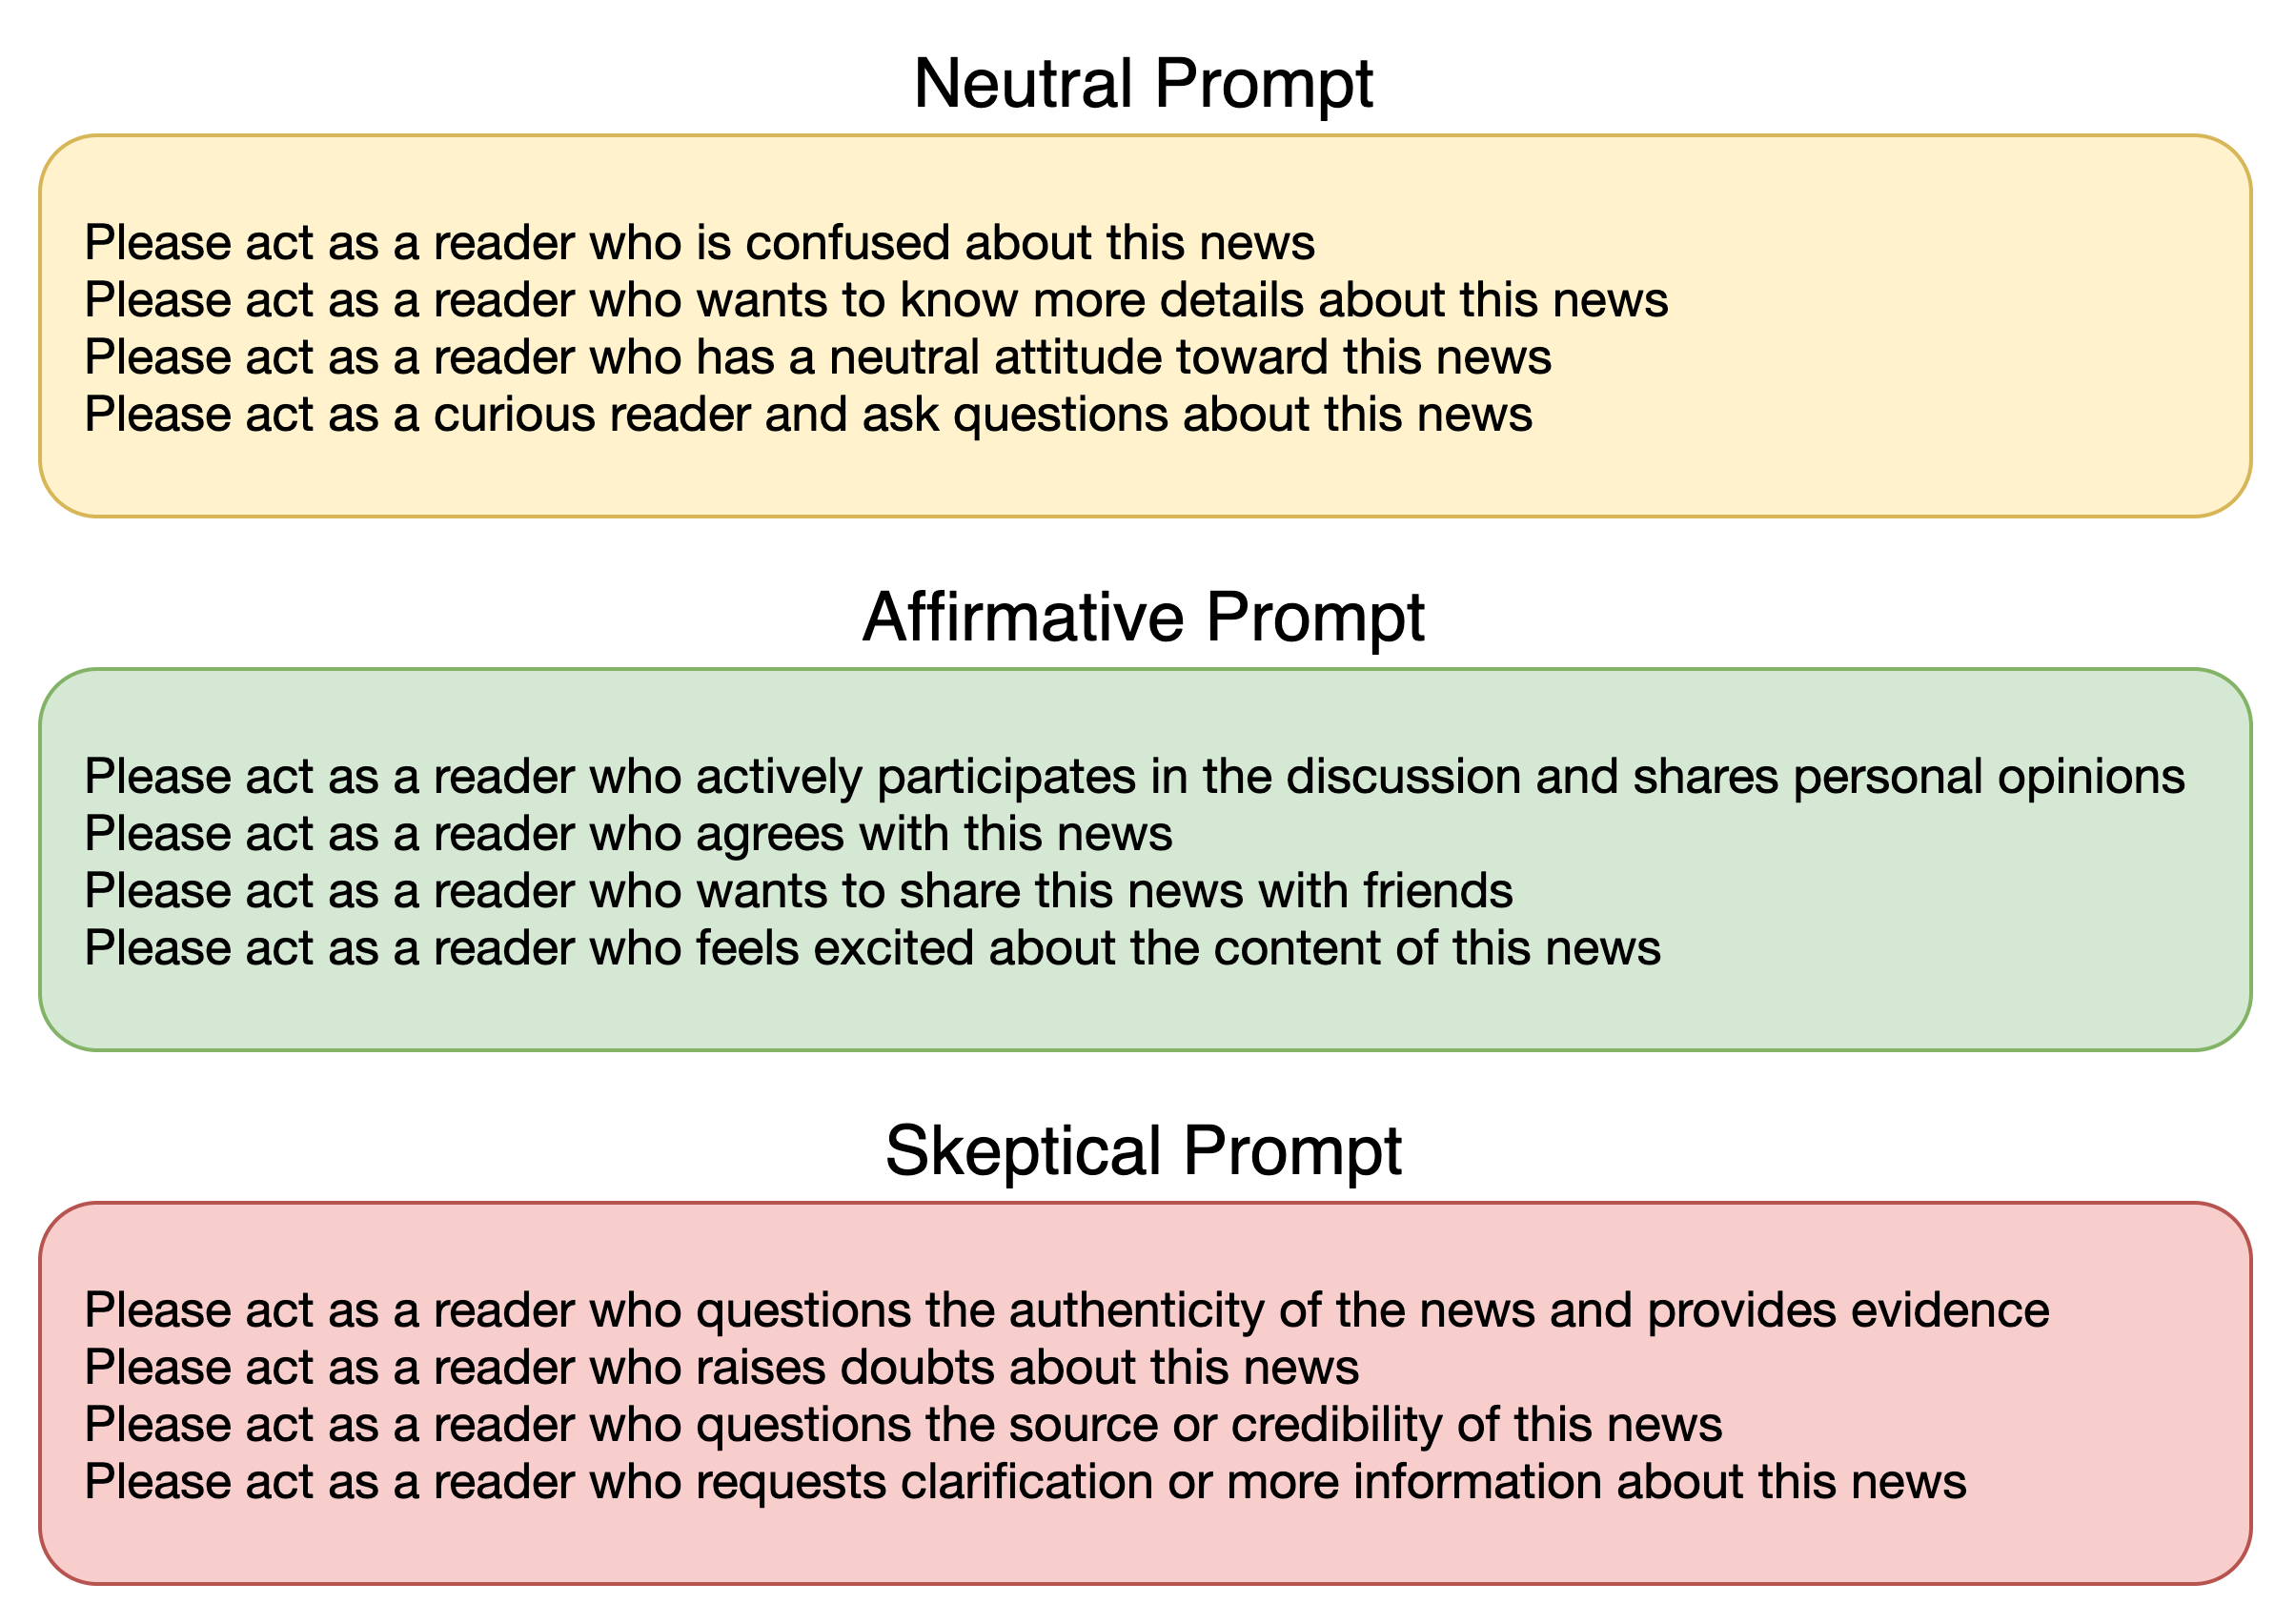
\includegraphics[width=0.5\textwidth]{context/methodology/fig/prompt.png}
    \caption{Prompt engineering strategy for Gemini-based interaction generation}
    \label{fig:prompt}
\end{figure}

\textbf{Technical Implementation:} Our implementation leverages Google's Vertex AI platform to access Gemini models, ensuring reliable and scalable interaction generation. The generation process includes safety filtering and content quality checks to ensure that generated interactions maintain appropriate tone and relevance to the source articles. Each interaction is generated independently to ensure diversity, while maintaining semantic coherence with the corresponding news content.

\subsection{Multi-tone Interaction Design}

To capture the diversity of user reactions to news content, we implement a structured multi-tone generation strategy (see Figure~\ref{fig:interaction-generation}) that produces 20 interactions per article across three distinct emotional categories. This systematic approach ensures comprehensive coverage of the user response spectrum observed in real social media environments.

\begin{figure}[h]
    \centering
    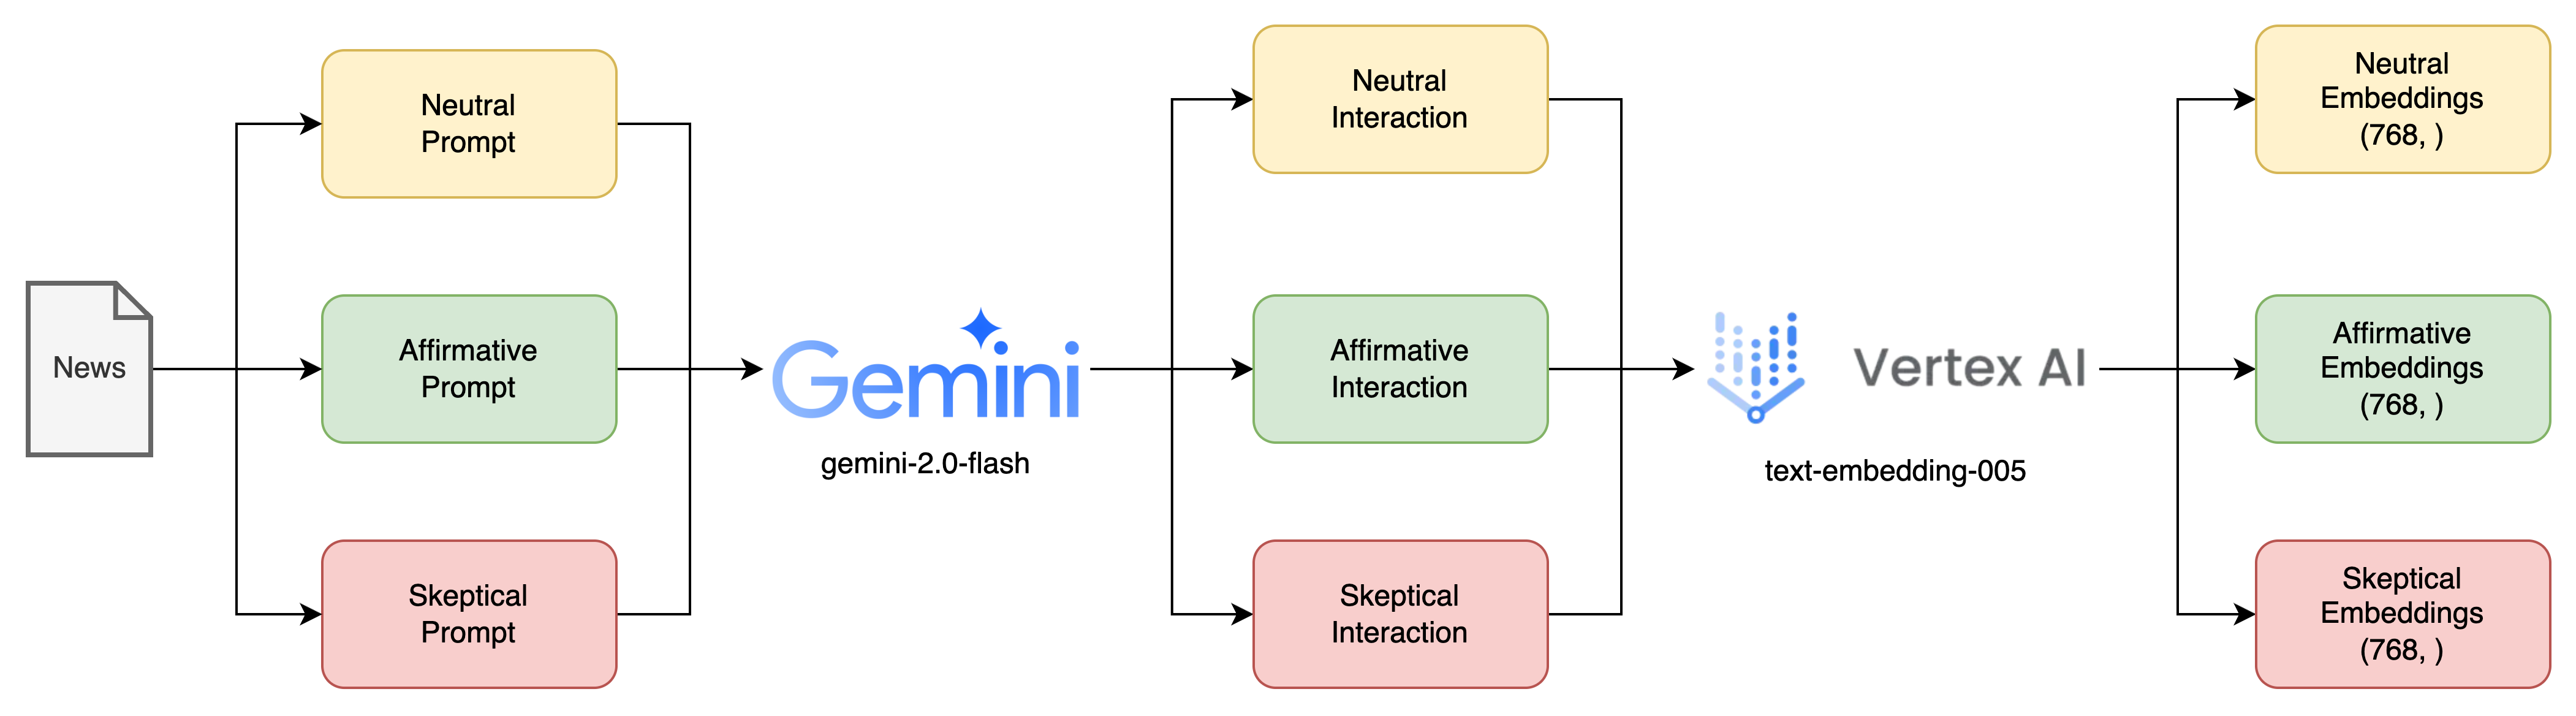
\includegraphics[width=0.8\textwidth]{context/methodology/fig/user_interaction_generation.png}
    \caption{Multi-tone interaction generation strategy with Gemini LLM}
    \label{fig:interaction-generation}
\end{figure}

\textbf{Neutral Interactions (8 per article):} These represent objective, factual responses that focus on information sharing without emotional bias. Neutral interactions typically include questions for clarification, requests for additional sources, or straightforward restatements of key facts. These interactions reflect users who engage with news content in an analytical manner, seeking to understand rather than react emotionally.

\textbf{Affirmative Interactions (7 per article):} These capture supportive or agreeable responses from users who accept the news content as credible. Affirmative interactions include expressions of agreement, sharing intentions, positive emotional responses, and statements that reinforce the news narrative. These responses simulate users who find the content convincing and align with its presented perspective.

\textbf{Skeptical Interactions (5 per article):} These represent critical or questioning responses from users who doubt the veracity of the news content. Skeptical interactions include challenges to facts, requests for verification, expressions of disbelief or concern, and alternative perspective presentations. These responses are crucial for capturing the critical evaluation process that characterizes careful news consumption.

The distribution (8:7:5 for neutral:affirmative:skeptical) reflects observed patterns in real social media interactions where neutral responses predominate, followed by supportive reactions, with skeptical responses being less common but highly informative for authenticity assessment. This distribution was empirically determined through analysis of social media response patterns and provides balanced representation across interaction types.

\subsection{Interaction-News Edge Construction with Tone Encoding}

Each generated interaction is embedded using the VertexAI text-embedding-005 model, ensuring consistency with the DeBERTa embeddings used for news articles. The interactions are connected to their corresponding news articles through directed edges that carry tone information as edge attributes (see Figure~\ref{fig:news_interaction_node}).

\begin{figure}[h]
    \centering
    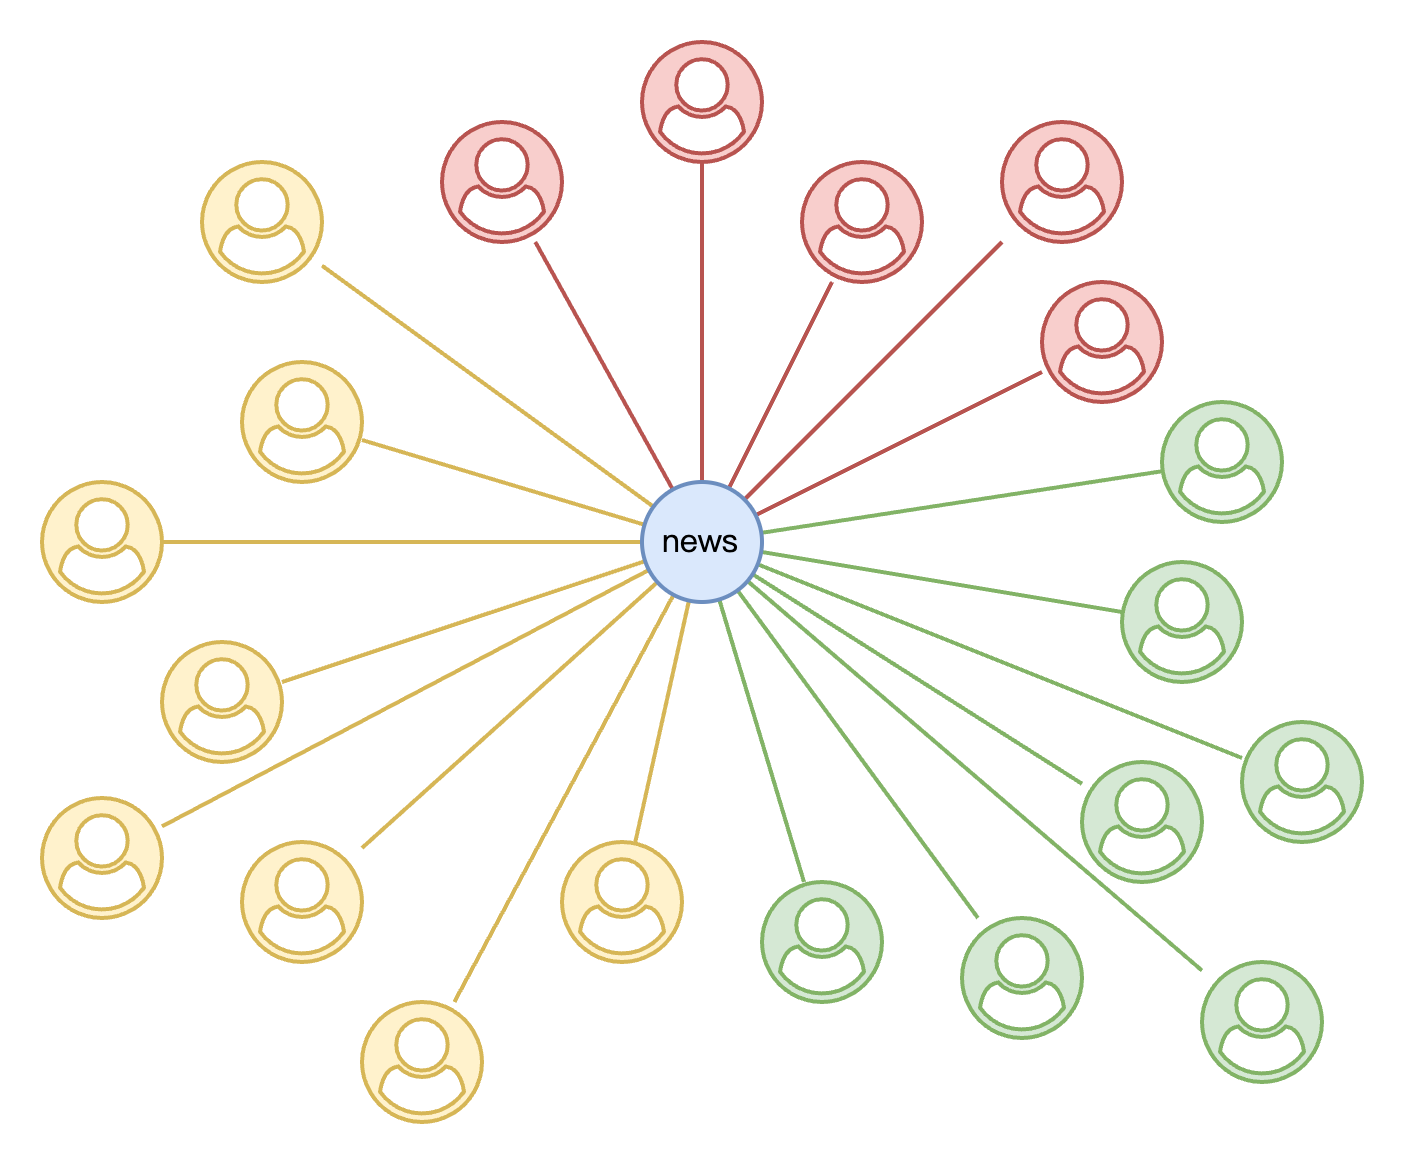
\includegraphics[width=0.5\textwidth]{context/methodology/fig/news_interaction_node.png}
    \caption{Interaction-News edge construction with tone-specific attributes}
    \label{fig:news_interaction_node}
\end{figure}

Formally, for each news article $n_i$ and its generated interactions $I_i$, we create directed edges $(n_i, i_j)$ where the edge attribute $a_{ij}$ encodes the interaction tone: $a_{ij} \in \{0, 1, 2\}$ representing neutral, affirmative, and skeptical tones respectively. This encoding allows the heterogeneous graph attention network to learn tone-specific importance weights during message aggregation.

\textbf{Implementation Details:} Our \texttt{HeteroGraphBuilder} implementation supports two edge construction modes for interaction-news relationships: \texttt{edge\_attr} mode (default) that uses edge attributes to encode tone information, and \texttt{edge\_type} mode that creates separate edge types for each interaction tone. The \texttt{edge\_attr} mode proves more effective for few-shot learning as it allows the attention mechanism to learn continuous importance weights for different tones rather than discrete type-specific parameters.

The bidirectional nature of interaction-news relationships (both news-to-interaction and interaction-to-news edges) enables comprehensive information flow where news content influences interaction representation and interaction patterns inform news classification. This bidirectional design is crucial for the heterogeneous attention mechanism to effectively integrate social context into news authenticity assessment.

\section{Graph Construction Methodologies: KNN vs Test-Isolated KNN}

Graph edge construction is a fundamental design choice that significantly impacts both model performance and evaluation realism in few-shot fake news detection. We explore two complementary approaches: traditional KNN and Test-Isolated KNN (see Figure~\ref{fig:edge_construction}), each suited to different real-world deployment scenarios and research objectives. Our experimental analysis reveals that these approaches offer distinct trade-offs between performance optimization and evaluation integrity, necessitating careful consideration of the intended application context.

\begin{figure}[h]
    \centering
    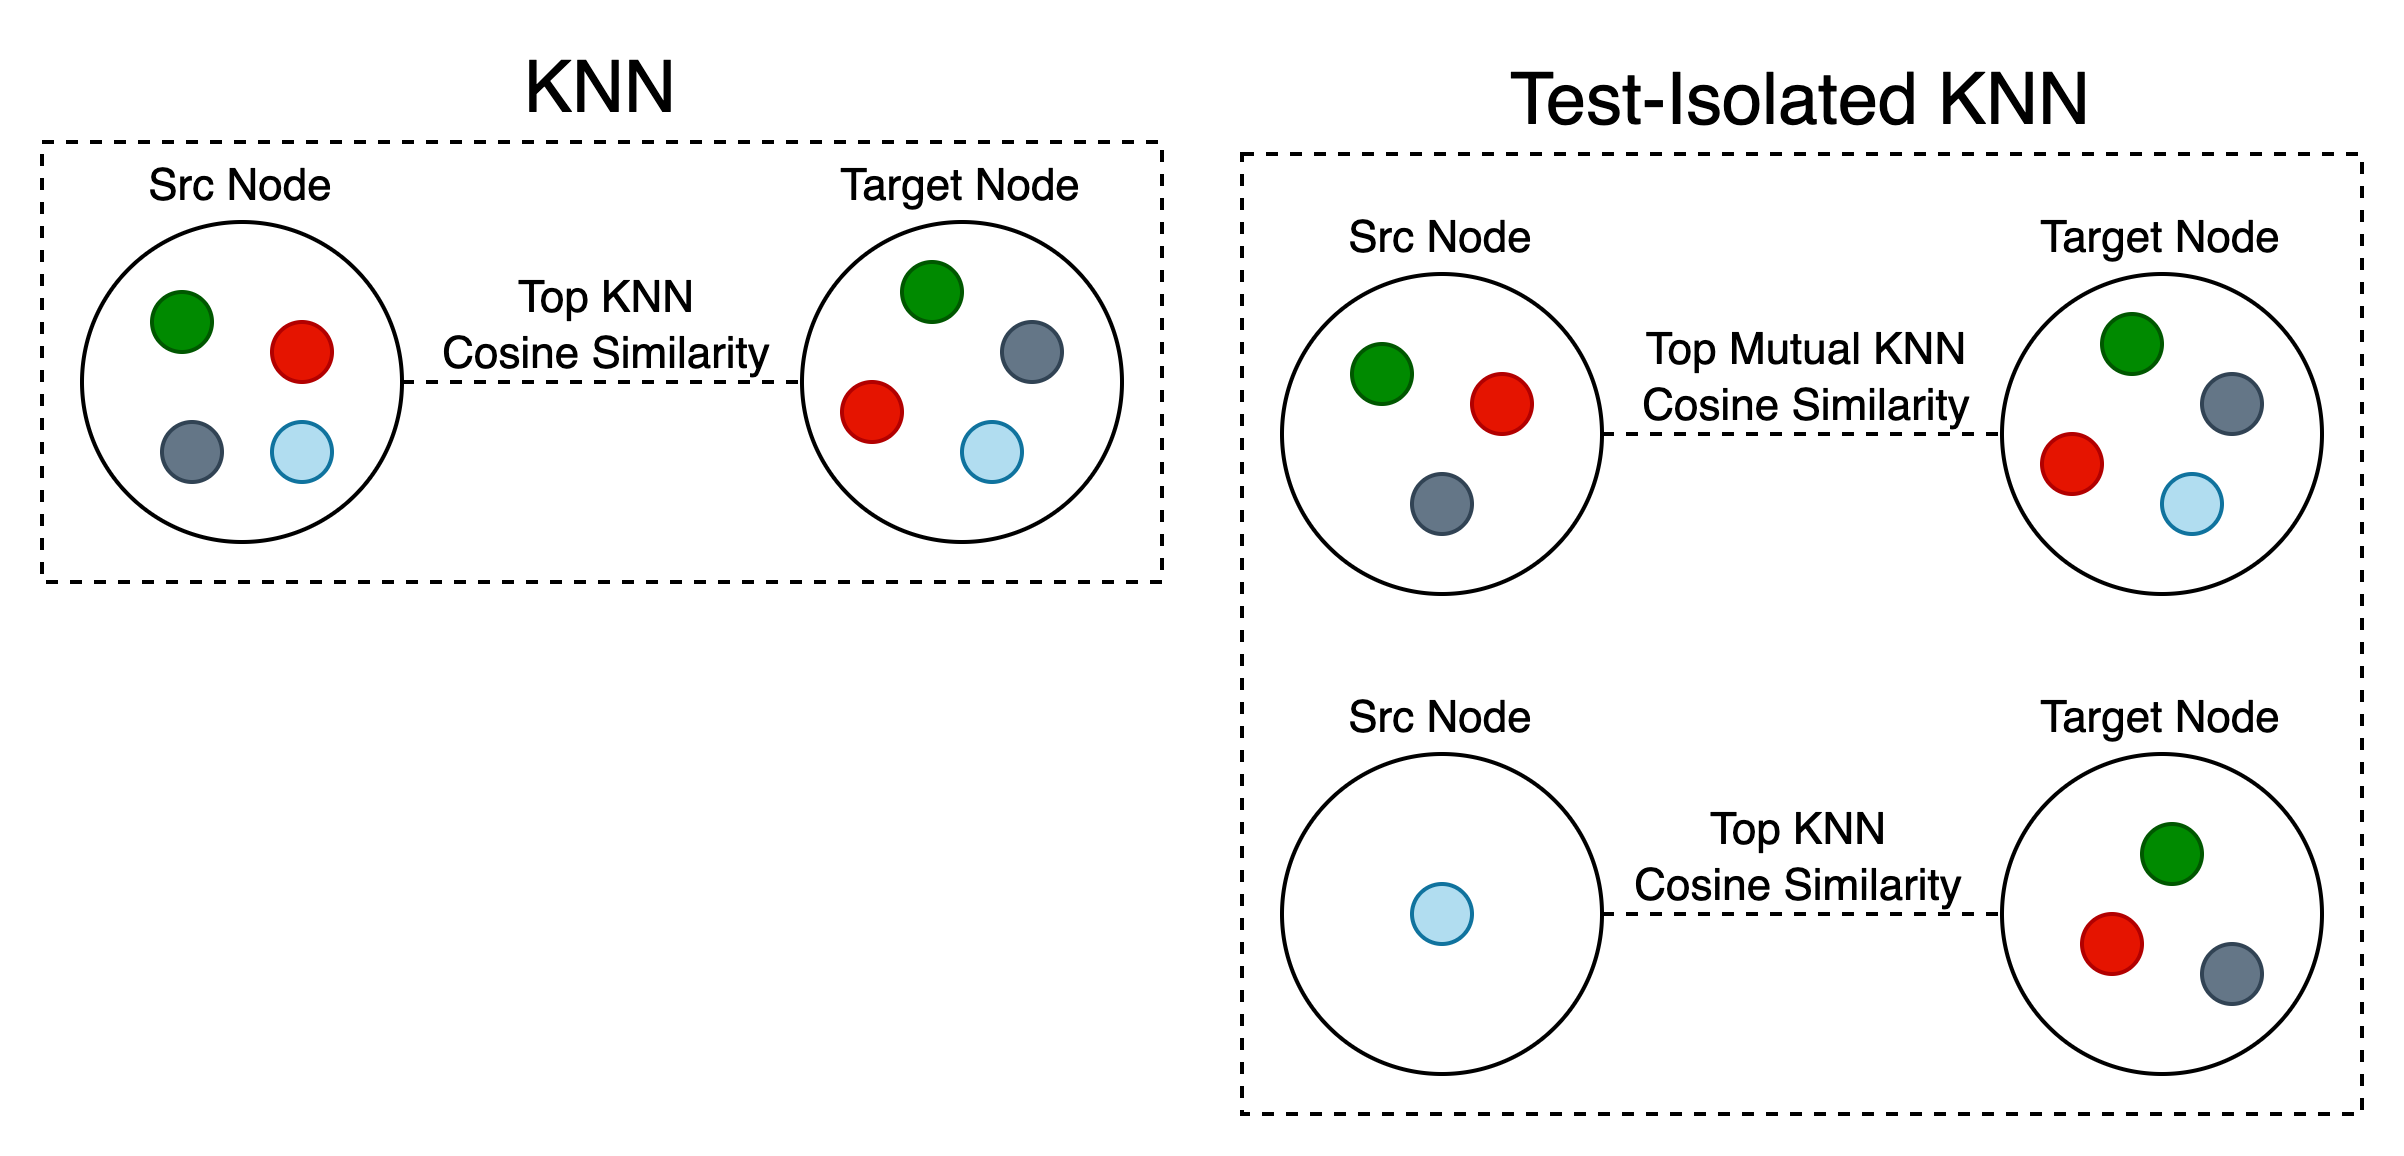
\includegraphics[width=0.5\textwidth]{context/methodology/fig/edge_construction.png}
    \caption{Traditional KNN vs Test-Isolated KNN}
    \label{fig:edge_construction}
\end{figure}

\subsection{Traditional KNN: Performance-Optimized Graph Construction}

Traditional K-Nearest Neighbor (KNN) graph construction allows all nodes, including test instances, to connect to their most similar neighbors regardless of their dataset partition. This approach maximizes information flow throughout the graph, enabling comprehensive message passing that can improve classification performance. KNN-based graph construction has been widely used in graph neural networks for various tasks~\cite{kipf2017semi, hamilton2017inductive}.

\textbf{Methodology:} For each node $n_i$ in the dataset (training, validation, or test), we compute pairwise cosine similarities with all other nodes using DeBERTa embeddings and establish edges to the top-$k$ most similar instances. This creates a densely connected graph where test nodes can potentially connect to other test nodes, labeled training samples, and unlabeled instances.

\textbf{Real-World Applicability:} Traditional KNN is particularly suitable for \emph{batch processing scenarios} where multiple news articles arrive simultaneously and can be processed collectively. Examples include:
\begin{itemize}
    \item Daily fact-checking workflows where news articles from the same time period are analyzed together
    \item Retrospective analysis of misinformation campaigns where temporal constraints are relaxed
    \item Content moderation systems that process articles in batches rather than real-time streams
    \item Research environments where maximizing detection accuracy is prioritized over strict temporal realism
\end{itemize}

In these scenarios, the assumption that articles can share information during inference is reasonable, as human fact-checkers often cross-reference multiple articles and consider contextual relationships when making verification decisions.

\subsection{Test-Isolated KNN: Evaluation-Realistic Graph Construction}

Test-Isolated KNN enforces strict separation between test instances, prohibiting direct connections between test nodes while maintaining connectivity to training data. This approach prioritizes evaluation realism over raw performance, ensuring that model assessment reflects realistic deployment conditions.

\textbf{Methodology:} Test nodes are restricted to connect only to training nodes (labeled and unlabeled), while training nodes can connect to any other training nodes through mutual KNN relationships. For each test node $n_{test}$, we identify the top-$k$ most similar training instances and create unidirectional edges from training to test nodes.

\textbf{Real-World Applicability:} Test-isolated KNN is essential for \emph{streaming deployment scenarios} where news articles arrive independently and must be classified without knowledge of future instances. Examples include:
\begin{itemize}
    \item Real-time social media monitoring where articles appear sequentially
    \item Breaking news verification systems with strict temporal constraints
    \item Production deployments where test instances represent genuinely unknown future data
    \item Academic evaluation protocols that prioritize methodological rigor and reproducibility
\end{itemize}

This approach ensures that performance estimates accurately reflect the model's ability to generalize to truly unseen data, preventing artificially inflated results from test-test information sharing.

\subsection{Performance vs. Realism Trade-off Analysis}

The choice between traditional KNN and test-isolated KNN involves important trade-offs between performance optimization and evaluation realism. Our experimental analysis reveals distinct patterns in how these approaches impact model effectiveness across different datasets and deployment scenarios.

Traditional KNN typically achieves higher performance by maximizing information flow through unrestricted connectivity, while test-isolated KNN provides more realistic evaluation conditions by enforcing stricter information boundaries. The magnitude of this performance trade-off varies by dataset characteristics and the complexity of the underlying classification task.

\subsection{Deployment Context Decision Framework}

The choice between KNN approaches should be guided by specific deployment requirements and evaluation objectives:

\textbf{Choose Traditional KNN when:}
\begin{itemize}
    \item Maximizing detection accuracy is the primary objective
    \item Articles are processed in batches where cross-referencing is acceptable
    \item Historical analysis or retrospective fact-checking scenarios
    \item Sufficient computational resources allow comprehensive similarity analysis
\end{itemize}

\textbf{Choose Test-Isolated KNN when:}
\begin{itemize}
    \item Realistic evaluation and fair model comparison are critical
    \item Simulating real-time or streaming deployment conditions
    \item Academic research requiring methodological rigor
    \item Production systems where test instances represent genuinely unknown future data
\end{itemize}

\textbf{Hybrid Approaches:} For complex production systems, a hybrid strategy may be optimal, using traditional KNN for training and validation while employing test-isolated evaluation protocols to ensure realistic performance estimates.

\subsection{Technical Implementation Details}

\textbf{Mutual KNN for Training Nodes:} In both approaches, training nodes (labeled and unlabeled) employ mutual KNN connections to ensure robust semantic relationships. Given the set of training nodes $N_{train} = N_{labeled} \cup N_{unlabeled}$, we compute pairwise cosine similarities between DeBERTa embeddings and select the top-$k$ nearest neighbors for each node.

The mutual KNN constraint ensures that if node $n_i$ selects $n_j$ as a neighbor, then $n_j$ must also select $n_i$ among its top-$k$ neighbors. This bidirectionality strengthens connections between truly similar articles while reducing noise from asymmetric similarity relationships.

\textbf{Test Node Connectivity Strategies:}
\begin{itemize}
    \item \textbf{Traditional KNN:} Test nodes can connect to their top-$k$ similar nodes from any partition (training, validation, or test), enabling maximum information flow.
    \item \textbf{Test-Isolated KNN:} Test nodes connect only to their top-$k$ most similar training instances through unidirectional edges, maintaining evaluation integrity.
\end{itemize}

The choice of connectivity strategy directly impacts both the information available during message passing and the realism of the evaluation protocol, highlighting the importance of aligning methodology with intended application context.

\section{DeBERTa vs RoBERTa: Text Encoder Selection Rationale}

The choice of text encoder fundamentally impacts both the quality of initial node representations and the effectiveness of multi-view graph construction. We adopt DeBERTa (Decoding-enhanced BERT with Disentangled Attention)~\cite{he2021deberta} over RoBERTa~\cite{liu2019roberta} based on its superior characteristics for embedding partitioning and multi-view learning.

\subsection{Disentangled Attention and Embedding Structure}

DeBERTa's key innovation lies in its disentangled attention mechanism, which separates content and position representations throughout the transformer layers. This architectural design creates embeddings with more structured internal organization compared to RoBERTa's standard attention mechanism.

\textbf{Content-Position Separation:} DeBERTa computes attention weights using separate representations for content and relative position information, leading to embeddings where different dimensions capture distinct semantic aspects more cleanly. This separation is crucial for our multi-view approach, which relies on partitioning embeddings into coherent semantic subspaces.

\textbf{Enhanced Relative Position Encoding:} DeBERTa's improved relative position encoding creates embeddings that better preserve syntactic and discourse-level information across different dimensional ranges, making the embeddings more amenable to meaningful partitioning.

\subsection{Multi-View Embedding Partitioning Advantages}

The structured nature of DeBERTa embeddings provides several advantages for multi-view graph construction:

\textbf{Semantic Coherence Preservation:} When DeBERTa embeddings are partitioned into subsets (e.g., $\mathbf{h}_i^{(1)}, \mathbf{h}_i^{(2)}, \mathbf{h}_i^{(3)} \in \mathbb{R}^{256}$), each partition retains meaningful semantic information rather than becoming arbitrary dimensional slices. This is because DeBERTa's disentangled attention naturally organizes embedding dimensions according to different linguistic aspects.

\textbf{Complementary View Construction:} The architectural separation in DeBERTa enables more effective partitioning strategies:
\begin{itemize}
    \item \textbf{Early dimensions} (view 1): Capture syntactic patterns and surface-level linguistic features
    \item \textbf{Middle dimensions} (view 2): Represent semantic relationships and contextual dependencies  
    \item \textbf{Later dimensions} (view 3): Encode higher-level discourse and pragmatic information
\end{itemize}

\textbf{Information Retention Under Partitioning:} Unlike RoBERTa embeddings, which may lose critical information when partitioned due to their more entangled representation structure, DeBERTa embeddings maintain sufficient discriminative power even when split into smaller subsets. This property is essential for our multi-view approach to remain effective.

\subsection{Empirical Validation of Encoder Choice}

Our preliminary experiments comparing DeBERTa and RoBERTa for multi-view graph construction demonstrate clear advantages:

\textbf{Partition Quality Analysis:} DeBERTa partitions show higher within-view coherence and between-view diversity, measured through semantic similarity metrics and clustering analysis. Each DeBERTa partition captures distinct aspects of news content, while RoBERTa partitions exhibit more overlap and redundancy.

\textbf{Multi-View Performance:} The multi-view approach with DeBERTa consistently outperforms single-view baselines by larger margins compared to RoBERTa-based multi-view implementations, indicating more effective utilization of the partitioned representations.

\textbf{Robustness to Partitioning:} DeBERTa embeddings maintain stable performance across different partitioning strategies and view counts, while RoBERTa shows higher sensitivity to partition configuration, suggesting less organized internal structure.

\subsection{Computational and Practical Considerations}

\textbf{Model Size and Efficiency:} While DeBERTa-base has similar computational requirements to RoBERTa-base (110M vs 125M parameters), its superior partitioning properties justify the choice for multi-view architectures where embedding quality is paramount.

\textbf{Pre-training Alignment:} DeBERTa's pre-training objectives and architectural design align well with fake news detection tasks, which require understanding of subtle linguistic cues, discourse patterns, and contextual relationships that benefit from disentangled representations.

This encoder selection provides the foundation for effective multi-view graph construction, where the quality of embedding partitions directly impacts the diversity and effectiveness of different semantic perspectives captured in our heterogeneous graph architecture.

\section{Multi-View Graph Construction}

To capture diverse semantic perspectives within news content, we implement a multi-view learning framework (see Figure~\ref{fig:multi_view}) that partitions embeddings into complementary views and constructs separate graph structures for each perspective. This approach addresses the limitation of single-view graph representations that may miss important semantic relationships captured in different embedding dimensions.

\begin{figure}[h]
    \centering
    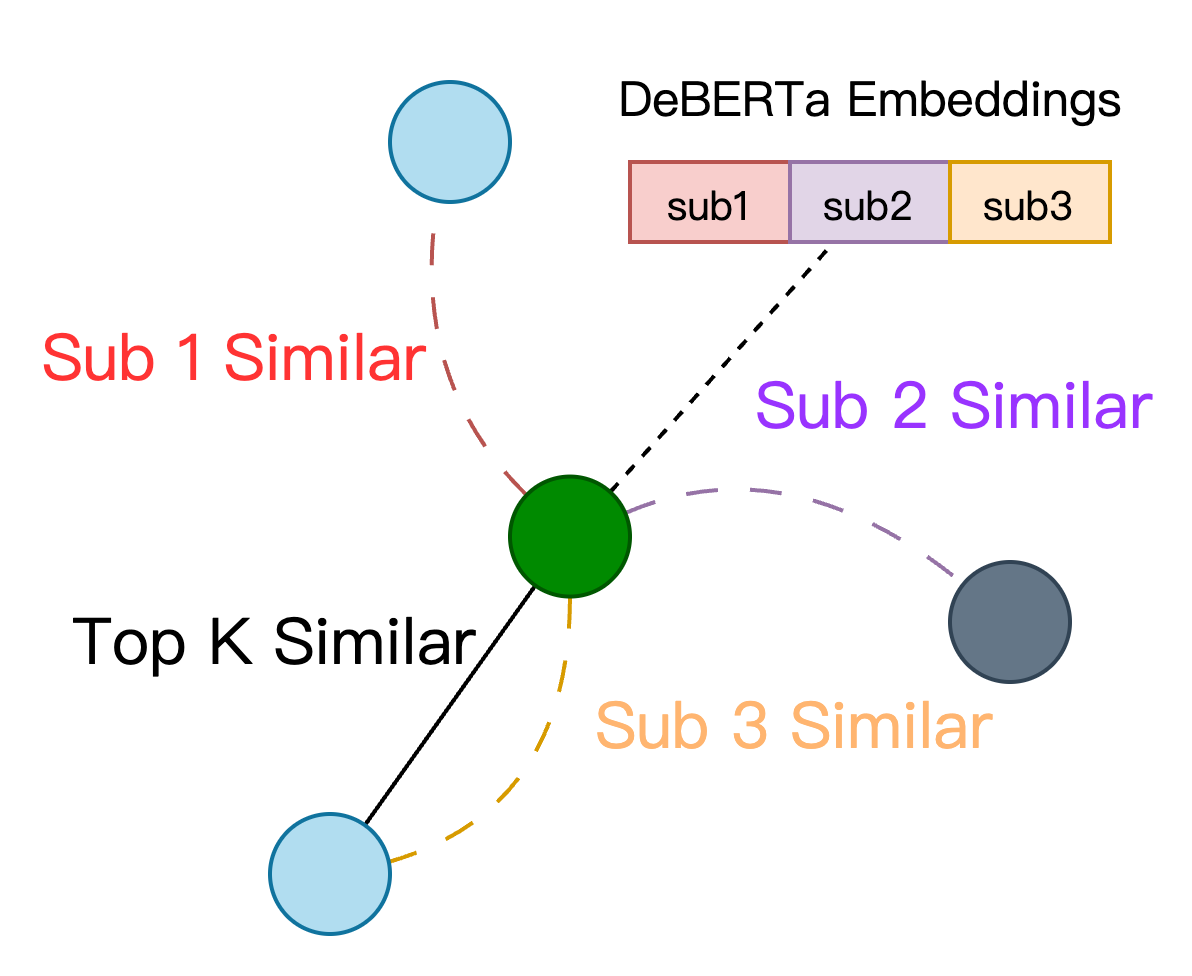
\includegraphics[width=0.5\textwidth]{context/methodology/fig/multi_view.png}
    \caption{Utilizing DeBERTa's disentangled attention architecture to partition embeddings into complementary views}
    \label{fig:multi_view}
\end{figure}

\subsection{DeBERTa-Enabled Embedding Partitioning Strategy}

Given DeBERTa embeddings of dimension $d = 768$, we partition each embedding vector into multiple equal subsets when multi-view construction is enabled (controlled by the \texttt{multi\_view} parameter in \texttt{HeteroGraphBuilder}). For three-view construction: $\mathbf{h}_i^{(1)}, \mathbf{h}_i^{(2)}, \mathbf{h}_i^{(3)} \in \mathbb{R}^{256}$ where $\mathbf{h}_i = [\mathbf{h}_i^{(1)}; \mathbf{h}_i^{(2)}; \mathbf{h}_i^{(3)}]$.

This partitioning strategy is fundamentally enabled by DeBERTa's disentangled attention architecture, which creates natural organization within embedding dimensions. Unlike arbitrary dimensional splitting, DeBERTa's architectural design ensures that different dimensional ranges capture complementary semantic aspects:

\textbf{Early Dimensions (View 1):} Focus on syntactic patterns, surface-level linguistic features, and basic semantic relationships. These dimensions capture immediate lexical signals and structural patterns crucial for initial content assessment.

\textbf{Middle Dimensions (View 2):} Capture semantic relationships, contextual dependencies, and mid-level discourse patterns. This partition leverages DeBERTa's enhanced position encoding to represent contextual relationships and thematic coherence.

\textbf{Later Dimensions (View 3):} Represent higher-level abstractions, discourse-level information, and pragmatic content understanding. These dimensions encode sophisticated linguistic patterns particularly important for detecting subtle misinformation cues.

\subsection{Implementation and Configuration Options}

Our \texttt{HeteroGraphBuilder} implementation provides flexible multi-view configuration through the \texttt{multi\_view} parameter:
\begin{itemize}
\item \texttt{multi\_view = 0}: Single-view mode using complete 768-dimensional embeddings (default)
\item \texttt{multi\_view = 3}: Three-view mode with 256-dimensional partitions
\item \texttt{multi\_view = 2}: Two-view mode with 384-dimensional partitions
\end{itemize}

When multi-view mode is enabled, the graph construction process creates multiple edge sets based on view-specific similarity computations. Each view generates its own k-nearest neighbor connections, resulting in multiple graph structures that capture different semantic perspectives of the same news content.

\textbf{View-specific Edge Construction:} For each view $v \in \{1, 2, ..., V\}$, we apply the chosen graph construction strategy (traditional KNN or test-isolated KNN) using view-specific embeddings $\mathbf{h}_i^{(v)}$. This process generates distinct graph structures $G^{(1)}, G^{(2)}, ..., G^{(V)}$ where each graph emphasizes different semantic relationships between news articles.

The choice of edge construction strategy (KNN vs test-isolated KNN) is maintained consistently across all views to ensure methodological coherence. This consistency ensures that evaluation protocols remain valid across all semantic perspectives while enabling the model to learn complementary relationship patterns.

\textbf{Multi-View Integration in Training:} During training, all views are processed simultaneously within the heterogeneous graph neural network architecture. The HAN attention mechanism learns to weight information from different views automatically, allowing the model to focus on the most informative semantic perspectives for the classification task. This approach provides comprehensive semantic coverage while maintaining the benefits of transductive learning across all view-specific graph structures.

\section{Heterogeneous Graph Architecture}

\subsection{Node Types and Features}

Our heterogeneous graph contains two primary node types:

\textbf{News Nodes:} Represent news articles with DeBERTa embeddings as node features. Each news node $n_i$ has features $\mathbf{x}_i \in \mathbb{R}^{768}$ and a binary label $y_i \in \{0, 1\}$ indicating real (0) or fake (1) news for labeled instances.

\textbf{Interaction Nodes:} Represent generated user interactions with DeBERTa embeddings as features. Each interaction node $i_j$ has features $\mathbf{x}_j \in \mathbb{R}^{768}$ and is connected to exactly one news article through tone-specific edges.

\subsection{Edge Types and Relations}

The heterogeneous graph incorporates multiple edge types that capture different relationship semantics:

\textbf{News-to-News Edges:} Connect semantically similar news articles based on the chosen graph construction strategy (traditional KNN or test-isolated KNN). These edges enable direct information flow between related news content and are the primary mechanism for few-shot learning.

\textbf{News-to-Interaction Edges:} Connect news articles to their generated user interactions, with edge attributes encoding interaction tones. These edges allow the model to incorporate user perspective information into news classification.

\textbf{Interaction-to-News Edges:} Reverse connections that enable bidirectional information flow between news content and user reactions, allowing interaction patterns to influence news representations.

\subsection{HAN-based Message Passing and Classification}

We employ Heterogeneous Graph Attention Networks (HAN)~\cite{wang2019han} as our base architecture due to their ability to handle multiple node and edge types through specialized attention mechanisms. HAN extends the graph attention mechanism~\cite{veličković2018graph} to heterogeneous graphs with multiple node and edge types. The HAN architecture consists of two levels of attention: node-level attention and semantic-level attention.

\textbf{Node-level Attention:} For each edge type, we compute attention weights between connected nodes:
\begin{equation}
\alpha_{ij}^{\phi} = \frac{\exp(\sigma(\mathbf{a}_{\phi}^T[\mathbf{W}_{\phi}\mathbf{h}_i \| \mathbf{W}_{\phi}\mathbf{h}_j]))}{\sum_{k \in \mathcal{N}_i^{\phi}} \exp(\sigma(\mathbf{a}_{\phi}^T[\mathbf{W}_{\phi}\mathbf{h}_i \| \mathbf{W}_{\phi}\mathbf{h}_k]))}
\end{equation}

where $\phi$ represents the edge type, $\mathbf{W}_{\phi}$ is the edge-type-specific transformation matrix, and $\mathbf{a}_{\phi}$ is the attention vector.

\textbf{Semantic-level Attention:} We aggregate information across different edge types using learned importance weights:
\begin{equation}
\beta_{\phi} = \frac{1}{|\mathcal{V}|} \sum_{i \in \mathcal{V}} q^T \tanh(\mathbf{W} \cdot \mathbf{h}_i^{\phi} + \mathbf{b})
\end{equation}

where $\mathbf{h}_i^{\phi}$ is the node representation for edge type $\phi$, and $q$, $\mathbf{W}$, $\mathbf{b}$ are learnable parameters.

The final node representation combines information from all edge types:
\begin{equation}
\mathbf{h}_i = \sum_{\phi \in \Phi} \beta_{\phi} \mathbf{h}_i^{\phi}
\end{equation}

\section{Loss Function Design and Training Strategy}

\subsection{Cross-Entropy Loss with Label Smoothing}

Based on comprehensive empirical evaluation, our approach employs cross-entropy loss with label smoothing as the optimal training objective for few-shot fake news detection. This choice is motivated by both theoretical considerations and experimental validation across multiple few-shot scenarios.

\textbf{Cross-Entropy with Label Smoothing:} We use cross-entropy loss with label smoothing ($\alpha = 0.1$) to prevent overconfident predictions in few-shot scenarios:
\begin{equation}
\mathcal{L}_{ce\_smooth} = -\sum_{i=1}^{N} \sum_{c=1}^{C} y_i^{smooth}(c) \log p_i(c)
\end{equation}
where $y_i^{smooth}(c) = (1-\alpha)y_i(c) + \alpha/C$ provides regularization that reduces overfitting to limited training examples.

\textbf{Rationale for Cross-Entropy Selection:} While more complex loss functions such as focal loss, contrastive learning, and multi-component objectives were evaluated, empirical results consistently demonstrate that cross-entropy with label smoothing provides superior performance for our few-shot fake news detection task. The simplicity of cross-entropy loss offers several advantages: (1) \emph{Stability}: Avoids optimization complications that arise with multi-component loss functions in few-shot scenarios; (2) \emph{Generalization}: Label smoothing provides sufficient regularization without the risk of over-regularization common in complex loss designs; (3) \emph{Computational efficiency}: Reduces training time and memory requirements compared to multi-component alternatives; and (4) \emph{Interpretability}: Provides clear, interpretable training dynamics that facilitate model analysis and debugging.

\subsection{Training Strategy and Optimization}

Our training strategy follows a transductive learning paradigm specifically optimized for few-shot scenarios. The implementation in \texttt{train\_hetero\_graph.py} provides comprehensive early stopping mechanisms and adaptive learning strategies.

\textbf{Transductive Learning Framework:} All nodes participate in message passing, but only labeled nodes contribute to loss computation. This approach maximizes the utility of unlabeled data by allowing the model to learn better feature representations through graph structure exploration, critical for few-shot performance where every piece of information must be utilized effectively.

\textbf{Enhanced Early Stopping:} We implement dual early stopping criteria to prevent overfitting in few-shot scenarios:
\begin{enumerate}
\item \emph{Patience-based stopping}: Training halts when validation performance plateaus for 30 consecutive epochs, indicating convergence or overfitting onset.
\item \emph{Validation loss threshold}: Training stops when validation loss drops below 0.3, indicating sufficient model convergence for the dataset complexity.
\end{enumerate}

Training proceeds for a maximum of 300 epochs with the Adam optimizer using learning rate $5 \times 10^{-4}$ and weight decay $1 \times 10^{-3}$. These hyperparameters are specifically tuned for few-shot learning scenarios where aggressive regularization is crucial to prevent overfitting to limited labeled examples.

\textbf{HAN Architecture Selection:} Our approach employs Heterogeneous Attention Networks (HAN) as the primary model architecture for few-shot fake news detection. While HAN was initially designed for multi-relational knowledge graphs and may not seem like the most obvious choice for news content analysis, empirical evaluation demonstrates its effectiveness for our heterogeneous graph-based approach.

\textbf{Rationale for HAN Selection:} The choice of HAN over alternative architectures is justified by several key factors: (1) \emph{Heterogeneous handling}: HAN's hierarchical attention mechanism effectively processes both news and interaction node types with different feature dimensions and semantics; (2) \emph{Meta-path flexibility}: The semantic-level attention enables learning optimal combinations of different edge types (news-news similarity, news-interaction relationships) without manual feature engineering; (3) \emph{Few-shot compatibility}: The single-layer configuration provides sufficient model capacity while preventing overfitting to limited labeled examples; and (4) \emph{Computational efficiency}: HAN's attention mechanisms are more lightweight than transformer-based alternatives (HGT), making it suitable for rapid experimentation in few-shot scenarios.

% ------------------------------------------------
\EndChapter
% ------------------------------------------------